\documentclass[12pt]{article}
\PassOptionsToPackage{quiet}{fontspec}
\usepackage[a4paper, total={6.5in, 10in}]{geometry}
\usepackage{amsmath}
\usepackage{tikz}
\usepackage{ctex}
\usepackage{pgfplots}
\pgfplotsset{compat=1.17}
\usepackage{xcolor}
\usepackage{float}
\usetikzlibrary {backgrounds, mindmap, trees, arrows.meta}
\usepackage{enumerate}

\newcommand{\scale}[2]{%
    \scalebox{#1}[#1]{#2}}

\title{mindmap绘制}
\author{Eureka}
\date{\today}
\begin{document}
\maketitle
\tableofcontents
\clearpage

\section{简单绘制}
只需要使用一个简单的tikz命令即可

\noindent\rule{.9\linewidth}{2pt}
\begin{verbatim}
\tikz[small mindmap, concept color=gray!30] 
    \node [concept] {Isolate node};
\end{verbatim}

\subsection{基本架构}
\begin{itemize}
    \item mindmapd样式大小:small(有时会出bug), (norm), large, huge
    \item mindmap中node指定格式必须为 concept
    \item 添加 child 子节点时指定伸展方向(角度)
    \item 根节点 node 遇到分号;时, 子节点群才截至
\end{itemize}

\subsection{使用举例}
{\bf <1>} 一个普通的孤立奇点mindmap,\quad \lower20pt
\hbox{\scale{.6}{\tikz[small mindmap, concept color=gray!30, font=\kaishu] \node [concept] {孤立 node};}}

{\bf <2>} 一个简单的思维图形
\begin{center}
    \scale{.75}{
    \tikz[small mindmap,concept color=red!50,text=white]
    \node [concept] {根节点}% 
        child[grow=right, concept color=blue!30!green] {node[concept] {子节点1}}
        child[grow=160, concept color=orange!30!blue] {node[concept] {子节点2}};}
\end{center}

{\bf <3>} 下面讲解时的思维导图(PS:导图样式可以自定义)
\begin{figure}[!htb]
    \centering
    \scale{.7}{
    \begin{tikzpicture}[%
            % 设置对齐和填充
            every node/.style={fill=gray!30,rounded corners},
            edge from parent/.style={blue!50,-{Circle[open]},very thick,draw},
            % 设置每一个层级之间的举例以及姊妹节点间距
            level 1/.style={level distance=25mm, sibling distance=55mm},
            level 2/.style={level distance=30mm, sibling distance=25mm},
            level 3/.style={level distance=35mm, sibling distance=10mm}
        ]
        % 这个root说明只能放在[]前面
        \node{MindMap} [edge from parent fork right, grow=right]
            % 控制每一层的childs的对齐方向
            child[right] { node {节点排布}
                child[right] {node {child 级别}
                    % 也可以单独在每一个node中填写 right=-18pt
                    child {node {every concept}}
                    child {node {root concept}}
                    child {node {level <n> concept}}
                }
                child[right] {node {concept 排布}
                    child {node {横(纵)向}}
                    child {node {圆周向}}
                }
            }
            child[right] { node {样式定制}
                    child {node {concept 字体}
                        child {node {字体大小}}
                        child {node {字体样式}}
                    }
                    child {node {concept 颜色}
                        child {node {concept颜色}}
                        child {node {connection颜色}}
                    }
                    child {node {connection设置}
                        child {node {单色}}
                        child {node {渐变}}
                    }
            };
    \end{tikzpicture}}
\end{figure}

% 自定义edge样式
% \begin{tikzpicture}[level distance=11mm, sibling distance=15mm,
%     edge from parent path=
%     {(\tikzparentnode.south) .. controls +(0,-.5) and +(0,.5)
%     .. (\tikzchildnode.north)}, very thick]
%     \node {root} 
%         child {node {left}}
%         child {node {right}
%         child {node {child}}
%         child {node {child}}
%     };
% \end{tikzpicture}


\clearpage
\section{节点样式修改}
由于mindmap的字体和颜色等样式全部都已经定义,所以你必须使用如下的语句
进行重定义的基本格式

\noindent\rule{.95\linewidth}{2pt}
\begin{verbatim}
root concept/.append style={font=\small, concept color=blue!8},
level 1 concept/.append style={every child/.style={concept color=blue!30},font=\bf}
\end{verbatim}

\subsection{参数说明}

\begin{enumerate}[(1)]
    \item 节点排布
        \begin{itemize}
            \item 节点层级:extra concept, every concept, root concept, level 1(n) concept
            \item 姐妹节点之间的角度:sibling distance=90
            \item 排布方式:edge from parent fork right, grow=right
            \item 圆周排布:clockwise from=0(圆周排布的起点),sibling angle(圆周排列间隔) 
            \item 横向排布:sibling distance\;(不适用)
        \end{itemize}    
    \item 样式定制
        \begin{itemize}
            \item 字体大小:font=\textbackslash small
            \item 字体样式:font=\textbackslash kaishu
            \item concept颜色:concept color=blue!8
            \item connection颜色:渐变 \& 自定义
        \end{itemize} 
    \item 设置节点的最小尺寸: minimum size = 20(以确保节点具有一定的大小,即使其内容很小或为空)
    \item 若父子届节点颜色不同,想让tikz颜色自然过渡({\bf 后面会解释原因}),可以使用如下的两种方法:
        \begin{itemize}
            \item 使用\textbackslash tikz选项,不使用tikzpicture环境时:只需分别指定父子节点的颜色(不能在之前统一声明)
            \item 使用tikzpicture环境时,给level (n)应用concept color 选项时,添加every concept选项:every child/.style={concept color=blue!30}
        \end{itemize}
\end{enumerate}

\clearpage
\subsection{使用案例}
\begin{figure}[!htb]
    \centering
    \scale{.7}{
    \begin{tikzpicture}[%
            root concept/.append style={concept color=red!20, font=\bf},
            level 1 concept/.append style={every child/.style={concept color=blue!30}, font=\kaishu},
            mindmap
        ]
        % 注意:没有结束之前所有的node后均不能加上分号;
        \node[concept] {根节点}
            child [grow=30] { node[concept] {子节点A}
                child [grow=-30, concept color=green!70] {node[concept] {子子节点 $A_1$}}
                child [grow=30, concept color=red!70] {node[concept] {子子节点 $A_2$}}
            }
            child [grow=-30] {node[concept] {子节点C}}
            child [grow=150] { node[concept] {子节点B}
                child [grow=210, concept color=green!70] {node[concept] {子子节点 $B_1$}}
                child [grow=150, concept color=red!70] {node[concept] {子子节点 $B_2$}}
            }
            child [grow=210] {node[concept] {子节点D}};
    \end{tikzpicture}}
    \caption{一个使用的例子}
    \label{一个使用的例子}
\end{figure}

    
\section{节点连接}

\subsection{Simple Connection}
在绘制各层节点的时候把每一个node命名, 然后使用pgfonlayer的background选项慢慢draw即可。
下面即为一个最小示例

\noindent\rule{.9\linewidth}{2pt}
\begin{verbatim}
% \usetikzlibrary {backgrounds,mindmap}
% 第一步:绘制mindmap
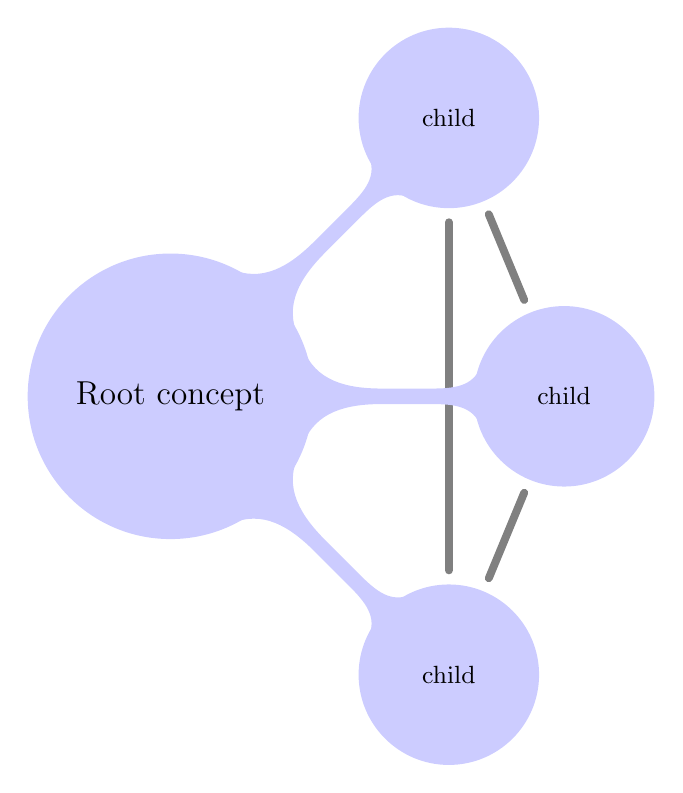
\begin{tikzpicture}[%
        root concept/.append style={concept color=blue!20,minimum size=2cm},
        level 1 concept/.append style={sibling angle=45},
        mindmap
    ]
    \node [concept] {Root concept}[clockwise from=45]
        child { node[concept] (c1) {child}}
        child { node[concept] (c2) {child}}
        child { node[concept] (c3) {child}};
    % 第二部:开始连线
    \begin{pgfonlayer}{background}
        \draw [concept connection] (c1) edge (c2)
                                        edge (c3)
                                   (c2) edge (c3);
    \end{pgfonlayer}
\end{tikzpicture}
\end{verbatim}

\begin{figure}[!htb]
    \centering
    % 第一步:绘制mindmap
    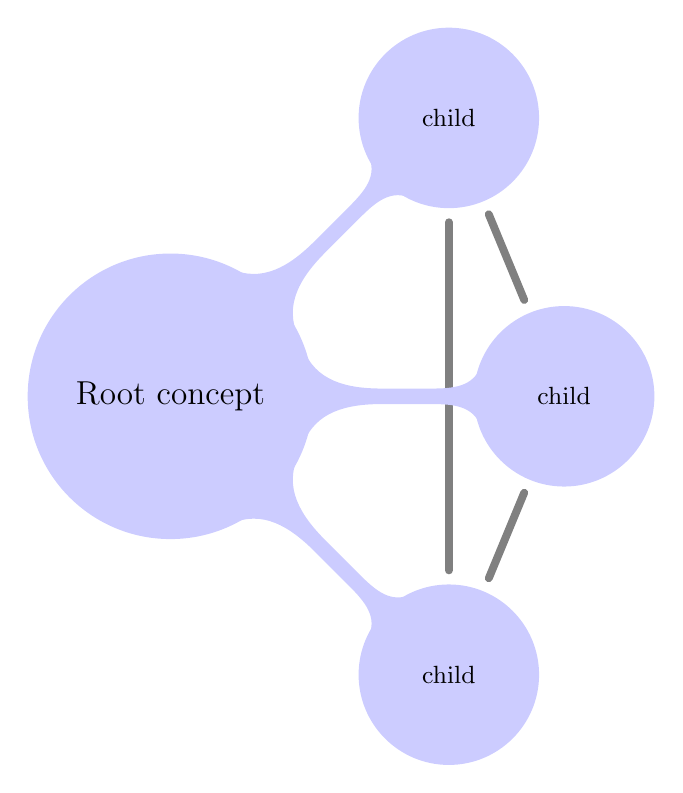
\begin{tikzpicture}[%
        root concept/.append style={concept color=blue!20,minimum size=1cm},
        level 1 concept/.append style={sibling angle=45},
        mindmap
    ]
    \node [concept] {Root concept}[clockwise from=45]
        child { node[concept] (c1) {child}}
        child { node[concept] (c2) {child}}
        child { node[concept] (c3) {child}};
    % 第二部:开始连线
    \begin{pgfonlayer}{background}
        \draw[concept connection] 
            (c1) edge (c2)
                 edge (c3)
            (c2) edge (c3);
    \end{pgfonlayer}
    \end{tikzpicture}
    \caption{默认样式}
    \label{默认样式}
\end{figure}


\subsection{The Circle Connection Bar}
各个调整参数的说明
\begin{enumerate}[(1)]
    \item start radius:其实半径
    \item end radius:结束半径
    \item amplitude:中间部分的矩形宽度
    \item angle:连接部分对应的圆心角
\end{enumerate}

下面先列举一个比较简单的例子来说明各个参数的实际意义:
\begin{figure}[!htb]
    \centering
    \scale{2.5}{
    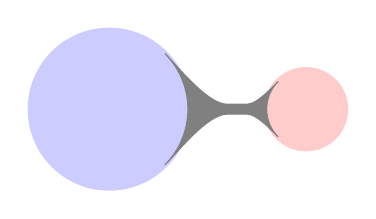
\begin{tikzpicture}[%
            decoration={start radius=1cm, end radius=.5cm, amplitude=1.25mm, angle=45},
            gray
        ]
        % 加一个1pt使得过渡更加的自然
        \fill[blue!20] (0,0) circle (1cm+1pt);
        \fill[red!20] (2.5,0) circle (.5cm+1pt);
        \filldraw [%
            % draw=red!60,
            % fill=gray,
            decorate,
            decoration=circle connection bar
        ] (1,0) -- (2,0);
    \end{tikzpicture}}
    \caption{简单例子}
    \label{简单例子}
\end{figure}


\clearpage
\subsection{The Circle Connection Bar To-Path}
这个万一就要稍微的复杂一丢丢了,
一个比较坑的就是:{\bf Require that the start and the target are circles.}
但是使用起来是比较简单的,但是仍然是直接一个
path (<node1>) to[circle connection bar] (<node2>)命令就行了.

mindmap默认使用的就是这种样式的connection, 而且concept color 选项会覆盖circle connection bar
switch colo选项,所以当我们分别设置了父子节点的颜色时,颜色会自动{\bf 渐变}.

具体的使用见下面命令:

\noindent\rule{.95\linewidth}{2pt}
\begin{verbatim}
% n1, n2 是前面已经定义的node名称
\path (n1) to[circle connection bar] (n2);
\end{verbatim}


\noindent{\bf <1>} 单色连接
\begin{figure}[!htb]
    \centering
    \scale{2}{
    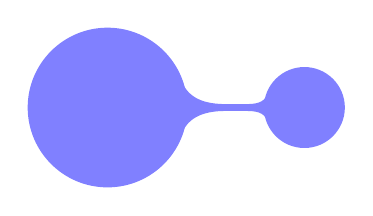
\begin{tikzpicture}[concept color=blue!50,blue!50,outer sep=0pt]
        \node (n1) at (0,0) [circle,minimum size=2cm,fill,draw,thick] {};
        \node (n2) at (2.5,0) [circle,minimum size=1cm,fill,draw,thick] {};
        \path (n1) to[circle connection bar] (n2);
    \end{tikzpicture}}
    \caption{Circle Connection}
    \label{Circle Connection}
\end{figure}

\noindent{\bf <2>} 渐变连接

mindmap还封装了颜色渐变,方便我们调用,
直接使用``函数'':circle connection bar switch color = from (<color1>) to (<color2>)

\begin{figure}[!htb]
    \centering
    \scale{2}{
    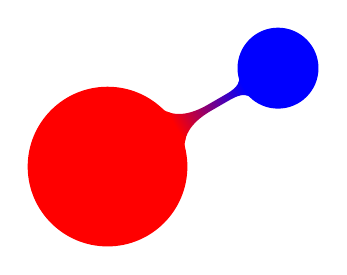
\begin{tikzpicture}[outer sep=0pt]
        \node (n1) at (0,0) [circle,minimum size=2cm,fill,draw,thick,red] {};
        \node (n2) at (30:2.5) [circle,minimum size=1cm,fill,draw,thick,blue] {};
        \path (n1) to[circle connection bar switch color=from (red) to (blue)] (n2);
    \end{tikzpicture}}
    \caption{颜色渐变}
    \label{颜色渐变}
\end{figure}

\section{添加标注}
这个是很简单的,但是标注(annotation)和extra concept 是不同的。
我们添加的标注无非就是给node指定一个annotation选项 

下面是一个二者的区别:
\begin{figure}[!htb]
    \centering
    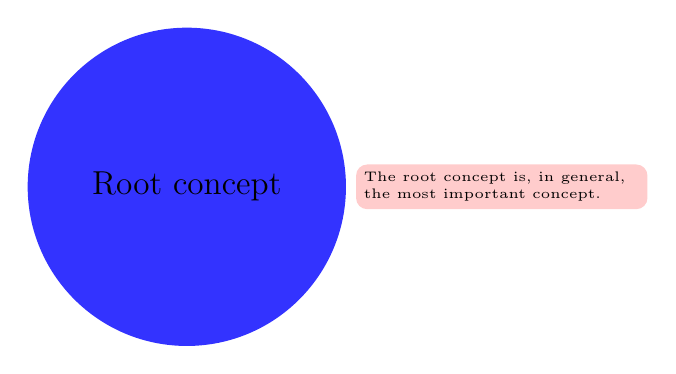
\begin{tikzpicture}[%
        mindmap,concept color=blue!80,
        every annotation/.style={fill=red!20}
    ]
        \node [concept] (root) {Root concept};
        \node [annotation, right] at (root.east)
            {The root concept is, in general, the most important concept.};
    \end{tikzpicture}
    \caption{difference between annotation and extra concept}
    \label{annotation and extra concept}
\end{figure}

\section{一个简单的应用作品}
\begin{figure}[!htb]
    \centering
    \scale{.8}{
    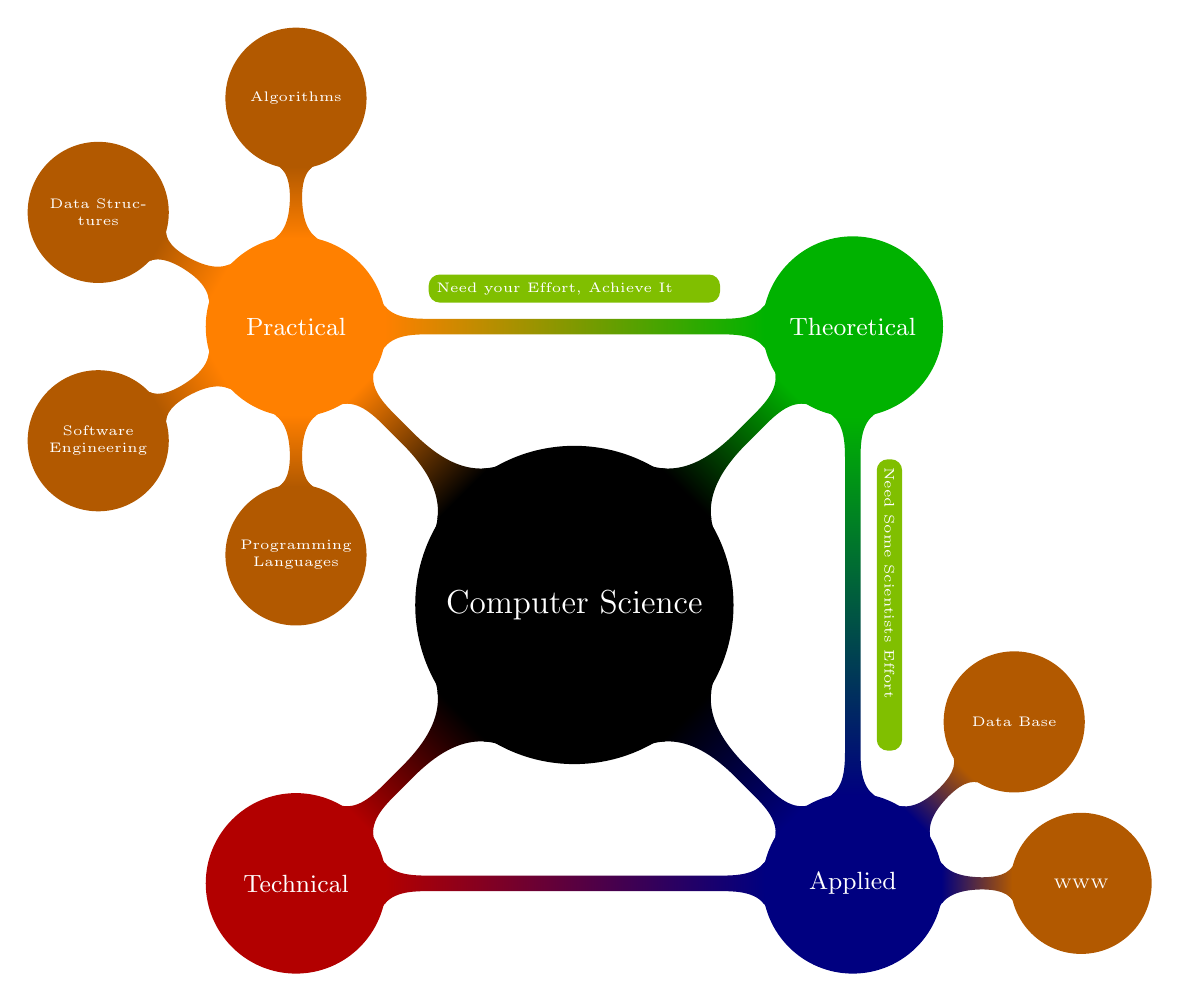
\begin{tikzpicture}[%
        mindmap,
        concept color=black,
        text=white, 
        level 2 concept/.append style={every child/.style={concept color=orange!70!black}, font=\tiny},
        every annotation/.style={fill=green!50!orange}   
    ]
        \node[concept] {Computer Science}
            child[grow=45, concept color=green!70!black] {node[concept] (theo) {Theoretical}}
            child[grow=225, concept color=red!70!black] {node[concept] (tec) {Technical}}
            child[grow=135, concept color=orange] {node[concept] (prac) {Practical}
                % 设置放置的起点为90,依次递减放置level 3的concept
                [clockwise from=-90]
                child {node[concept] {Pro\-gramming Languages}} 
                child {node[concept] {Software Engineering}}
                child {node[concept] {Data Structures}}
                child {node[concept] {Algorithms}}
            }
            child[grow=-45, concept color=blue!50!black] {node[concept] (app) {Applied}
                child [grow=45] {node[concept] {Data Base}}
                child [grow=right] {node[concept] {WWW}}
            };
        % 开始连线
        \path (theo) to[circle connection bar switch color=from (green!70!black) to (orange)] (prac);
        \path (theo) to[circle connection bar switch color=from (green!70!black) to (blue!50!black)] (app);
        \path (tec) to[circle connection bar switch color=from (red!70!black) to (blue!50!black)] (app);
        % 开始添加标注
        % child中的node不支持path 的 \path (node1) -- node[]{} (node2);操作
        \path (theo) node [midway,annotation,above=105pt]{Need your Effort, Achieve It} to (prac);
        \path (theo) node [midway,annotation,rotate=-90,above=105pt]{Need Some Scientists Effort} to (app);
    \end{tikzpicture}}
    \caption{作品}
    \label{作品}
\end{figure}


\section{结语}

以上就是tikz绘制mindmap的指导,挺简单的\; ???
是不是突然发现还是现成的思维导图软件香\; ???
巧了,我也这样觉得 !!!


\vspace*{2em}
\noindent\rule{.95\linewidth}{2pt}

参考:{\rmfamily {\bf[Till Tantau]} The TikZ and PGF Packages \texttt{Manual for version 3.1.8b} }

\end{document}